%
% Chapter 5
%

\chapter{FINAL REMARKS AND FUTURE OUTLOOK}

\section{Impact of Presented Lifetime Measurements}
Aside from the overall contribution of the lifetimes presented in this work in the global systematics of rare-earth structure, each isotope has local, isotopic significance and impetus for the measurement of nuclear lifetimes. The measurement of level lifetimes and corresponding reduced transition probabilities has been invaluable in understanding the structure of these nuclei in this geometric model, especially in terms of the new lifetimes of 0$^+$ excitations and new characterizations of vibrational states in deformed nuclei. 
\subsection{$^{160}$Gd}
Gadolinium-160 lies at the end of the road (figuratively) of decades long research on the structure of Gd isotopes; following the pioneering and continuing experimental works by Lesher, Aprahamian, de Haan, and others in $^{154-158}$Gd \cite{Lesher_158Gdmain,Jentschel_156Gd_GRID,Meyer_pt0_2006}, $^{160}$Gd lifetimes act as a capstone to understanding nuclear structure at the edges of the valley of stability, as well as structure at the limits of stable prolate deformation. Careful examination of our data has narrowed the focus of the systematic and on-going study of 0$^+$ excitations in the region, as we ruled out two possible states and measured key lifetimes for the remaining two K$^\pi$=0$^+$ bands. Invaluable knowledge on the characteristics of low-lying negative parity bands and K$^\pi$=4$^+$ bands was also gathered from our data, which opened the possibility of observing octupole and hexadecapole vibrations in deformed nuclei. Specifically, we observed a potential candidate for a collective $\beta$-vibration existing as the lowest 0$^+$ excitation at 1379~keV, and a well-defined two-phonon, K$^\pi$=0$^+$ $\gamma\gamma$ vibration for the other known 0$^+$ at 1558~keV. In contrast, we have not identified the K$^\pi$=4$^+$ branch of the $\gamma\gamma$ vibration in $^{160}$Gd, but confirm the well-behaved K$^\pi$=2$^+_\gamma$ band as a $\gamma$-type vibration with characteristically collective decays to the ground state. We have also identified several negative parity bands surmised to be a part of the octupole vibration through our measurement of collective B(E1) transition probabilities in the K$^\pi$=0$^-$ and 1$^-$ bands. Furthermore, we have observed collective decays from the K$^\pi$=2$^-$ band to the $\gamma$-vibrational band in an emerging trend in the rare-earth region \cite{Pascu_octupole_2015}.
\subsection{$^{162}$Dy}
The fact that the 47 new $^{162}$Dy lifetimes presented make is that these measurements account for a $\sim$0.2\% increase to the number of \textit{all} known literature lifetimes across \textit{all} 3000+ nuclei in existence. Putting this figure into even greater context, the 84 literature lifetimes for $^{168}$Er were gathered from extremely high resolution and efficiency detector arrays and spread across decades of experiments around the globe. With a single detector and a modestly discriminating spin population (J$^\pi\leq$5$^\pm$), we are able to provide a comparable number of lifetimes in $^{162}$Dy, putting it near the top of the list of experimentally measured lifetimes of excited states, not only in the rare-earth region, but across the entire Chart of Nuclides. In addition, if the overall complexity of DSAM-INS experiments and data analysis at UKAL are compared to other lifetime measurements around the globe, it is clear that DSAM-INS is an \textit{extremely} cost-efficient process and low barrier of entry to the experimentalist. The efficiency of cost stems from the single-detector setup with modest electronics required for signal processing, in comparison to the robust coincidence measurements needed elsewhere, and the straightforward analysis routines lend a veritable swiftness to the time required to publish results. Overall, several vibrational phenomena have been identified in $^{162}$Dy, with a K$^\pi$=0$^+$ $\gamma\gamma$-vibration as the lowest-lying 0$^+$ band at 1400~keV, along with two K$^\pi$=4$^+$ $\gamma\gamma$-vibrations at E$_{\rm x}$=1535 and 2181~keV excitation energy, in a first-of-its-kind measurement of both flavors of two-phonon $\gamma$ vibration. Much like the case for $^{160}$Gd, octupole vibrational characteristics have been identified that compliment the literature B(E3) transition probabilities that exist in the K$^\pi$=0$^-$ band, as well as two K$^\pi$=2$^-\rightarrow$2$^+_\gamma$ band decays; this trend of potential 2$^+\otimes$3$^-$ octupole-quadrupole vibration needs further study, but some key collective properties of these states has been uncovered.
\section{What Lies Ahead for Rare-Earth Nuclei?}
To reiterate the concerns of \cite{RevModPhys.83.1467} on the nature of any possible quadrupole vibrations in deformed nuclei, the successful measurement of two-nucleon transfer reaction cross sections, absolute B(E2) values (which have been substantially augmented with this work), and the $\rho^2$(E0) strengths is imperative. The spearheaded efforts by \cite{Meyer_pt0_2006} and this work cover the first two criteria, with the most elusive and experimentally exhaustive work remaining to measure E0 transitions. Fortunately, measurement of these crucial internal conversion electrons is possible at the Nuclear Science Laboratory at the University of Notre Dame du Lac, with the Internal Conversion Electron BALL array (ICEBALL). Using coincidence measurements of multiple Germanium detectors and charged particle Lithium-drifted Silicon detectors (SiLi), conversion electron strengths can be measured through careful electronics gates. The preferred mode of excitation at the NSL is via a ($\alpha$,2n) reaction for its preferential selection of postitive parity, L=0 and L=2 states. The ($\alpha$,2n) reaction also provides a secondary particle gate for proper event discrimination, with the implementation of triple-coincidence measurements being open (\textit{e.g.} one can trigger on a Germanium detector, a SiLi detector, \textit{and} a neutron detector, if desired).

In the specific case of $^{160}$Gd, this $\alpha$ implantation reaction proves difficult, as the preferred target required must be stable, and no suitable candidates apply ($^{158}$Sm is unstable). The feasibility of using other reaction channels is discouraging from a cross-section standpoint; the (n,$\alpha$) reaction cross section is well below a few microbarns ($\mu$b) for MeV-range incident neutrons that would be extracted from the on-site Tandem accelerator at the NSL. Complicate this problem further with the current lack of neutron production capabilities at the NSL, and the successful measurement of E0 transitions begins to seem less realistic.

For $^{162}$Dy, however, measurement of E0 transitions is readily possible at the NSL via the ($\alpha$,2n) reaction; incidentally and ironically, the backed targets used in ICEBALL experiments require a modest natural abundance of the particular isotope, in this case ironically, $^{160}$Gd. Looking forward, E0 measurements could be a feasible experiment at Notre Dame in the very near future, and is worthwhile to carry out experiments of this type to continue research on the structurally rich $^{162}$Dy.

To complete the picture of the evolution of nuclear structure in the rare-earth region, the measurement of absolute B(E2) transition probabilities for other nuclei would be ideal. This can be done for a modest number of the even-even Gd, Er, and Yb isotopes, yet distinct challenges arise in the feasability of acquiring enough target material to perform DSAM measurements for other Dysprosium nuclei. A very large portion of the natural abundances of Dy nuclei is split between the odd-A isotopes; this poses a problem that would force either an (n,$\gamma$) reaction (not ideal because of the inherent neutron backgrounds) to be used, and that target production could become increasingly expensive. Piled on top of this, target purity greatly affects the reliability of lifetimes measured with DSAM, where we utilize very large quantities of $>$95\% enriched oxide powders, but in lower quality targets, this enrichment would be severely impacted by the lack of natural abundances in certain isotopes.

As a supplement, refinement of lifetimes in the $^{160}$Gd and $^{162}$Dy is entirely possible and more than welcome in the cases where we can only measure lower limits for the lifetime. Luckily, methods to measure lifetimes in the super-picosecond range is achievable with the techniques mentioned in \S \ref{sec:lifetime_measurement_techniques} such as GRID or Coulomb Excitation. Along the same lines in terms of the refinement of spectroscopy of the nuclei studied in this work, five (5) tentative and confirmed 0$^+$ excitations by \cite{Meyer_pt0_2006} were not observed in our (n,n$^\prime\gamma$) experiments; these states could be probed further at the University of Notre Dame via ($\alpha$, $\alpha^\prime\gamma$) reactions with high-efficiency detectors in regular use in the lab (GEORGINA). Doing this removes certain, unfortunate, backgrounds (namely the (n,$\gamma$) humps that prevent the detection of the tentative 0$^+$ at 774.2~keV), and allows a much higher detection probability for much lower intensity $\gamma$ rays. The precise coincidence measurements of $\gamma$ rays stressed in \S \ref{sec:162Dy_0s_gamma} can also be done at the Nuclear Science Laboratory with multi-detector arrays like GEORGINA, further aiding the campaign to fully understand the nature of 0$^+$ excitations.

Since many rare-earth nuclei exist at the limits of a rotational, deformed shape, and that there is such a variation in the interpretation of the lowest-lying 0$^+$ states in the region, there may be latent trends hidden in the systematics of the states to further investigate. Figure \ref{fig:Rare_earth_E02} shows the energy of the 0$^+_2$ states in deformed rare-earth nuclei as a function of A (and N). Of note, we notice the sharp drop in energy for Samarium nuclei as deformation rapidly takes hold, with a somewhat local peak in energy around the $^{166,168}$Er isotopes, followed by another downward trend for Ytterbium and Hafnium nuclei. Experimentally, the lifetimes of 0$^+$ bands in this local area are far from complete, as we only have concrete evidence for $\gamma\gamma$-type vibrations existing in the Erbium nuclei (as the second and fifth 0$^+$). One question we want to ask is: does this local peaking of energy correlate to a different interpretation of the lowest-lying 0$^+$ state? There may \textit{not} be a connection between the energy of the state and its makeup, however, without proper spectroscopy (including absolute B(E2) measurements), the question remains open, and perhaps this sparks a new interest in some targeted areas of rare-earth nuclei. On the same subject, Figure \ref{fig:Rare_earth_02_BE2} shows the current status of absolute B(E2) measurements for the 0$^+_2\rightarrow$2$^+_{gs}$ transitions as a function of A, which is not only a sparsely populated figure, but also scattered across orders of magnitude of B(E2) strength. 

\begin{figure}[h!]
\begin{center}
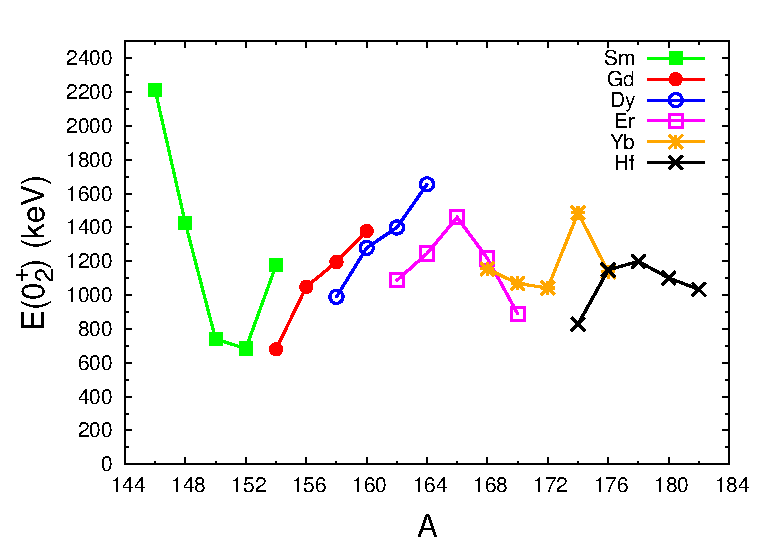
\includegraphics[width=0.95\textwidth]{figures/Rare_Earth_0s_energies.eps}\\
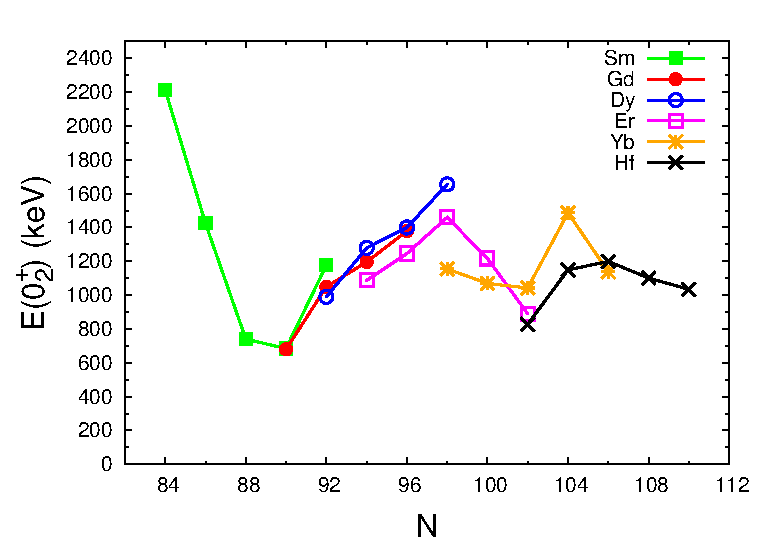
\includegraphics[width=0.95\textwidth]{figures/Rare_Earth_0s_N.eps}\\
\end{center}
\caption{Energies of the lowest-lying 0$^+$ state as a function of A (top) and N (bottom) for rare earth Sm, Gd, Dy, Er, Yb and Hf isotopes. \label{fig:Rare_earth_E02}}
\end{figure}

\begin{figure}[h!]
\begin{center}
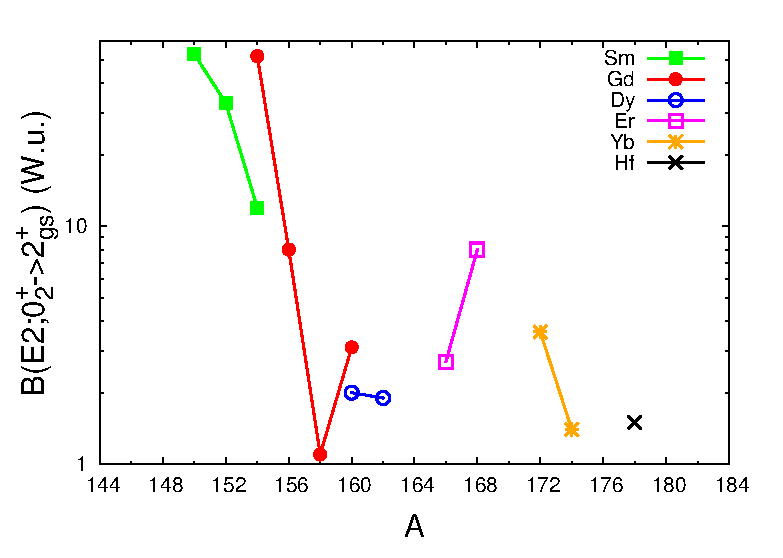
\includegraphics[width=0.95\textwidth]{figures/Rare_Earth_02_BE2.eps}
\end{center}
\caption{Known experimental B(E2) strengths of the lowest-lying 0$^+$ state as a function of A for rare earth Sm, Gd, Dy, Er, Yb and Hf isotopes. \label{fig:Rare_earth_02_BE2}}
\end{figure}

Finally, the stage is set for more lifetime measurements to be made (especially for the excited 0$^+$ states found in \cite{Meyer_pt0_2006}) for the vast set of rare-earth nuclei. The systematic pictures shown in \S \ref{sec:Structure_systematics} arise again, where we notice a complete paucity of lifetime information for these 0$^+$ excitations (namely $^{166,168}$Er and $^{154,156}$Gd). These lifetimes have furthered the elucidation of single \& double phonon vibrations in deformed nuclei, but ``there is always work to do" in the rare-earth region of nuclei, as the mystery of many structure phenomena is far from clear or well understood.
% \cite{Spiecker_E1strength}
% \cite{Aprahamian2002}
% \cite{Aprahamian200642}
% \cite{Aprahamian2004}
% \cite{Bender_pairing2000}
% \cite{Borner_collective1999}
% \cite{Casten_deformation1981}
% \cite{Chakraborty_negparity2012}
% \cite{Gibson_BlockingLifetimes1975}
% \cite{Clark_pairtransfer2009}
% \cite{Garrett_DSAM_INS2000}
% \cite{GRAETZER19661}
% \cite{Gupta_BE2quad2014}
% \cite{Honig_5minus1969}
% \cite{JAMMARI_1988}
% \cite{Lovhoiden_160pt}
% \cite{McGowan_BE2_1981}
% \cite{Meyer_pt0_2006}
% \cite{NEERGARD197033}
% \cite{PIEPENBRING_negpar_1991}
% \cite{Pietrella_beta_2004}
% \cite{SharpeySchafer_beta2011}
% \cite{Lesher_158Gdmain}
% \cite{WINTERBON_1975}
% \cite{Wu_2minus_2001}
% \cite{WuAprahamian_multiphonon_1994}
% \cite{Zamfir_162Dy0_1999}
% \cite{Zilges_K0dipole}
% \cite{Wong_text}
% \cite{Casten_text}
% \cite{BohrMott_text}
% \cite{Koning_OMP_2002}